\documentclass{paper}
\usepackage{minted}
\usepackage{tikz}
\newcommand{\drawEdge}[5]{
  \draw[->] (#1) to[#5] node[midway, above] (#3Above) {$#4$} (#2);
  \draw[->] (#1) to[#5] node[midway, below] (#3Below) {} (#2);
}
\begin{document}

\section*{Intension}
I've seen various introduction about monad, but none of them is clear enough for me to understand. So I decided to write my own introduction about monad.
To understand monad in programming is not difficult, but it is complex. We need to understand a lot of smaller concepts before we can understand monad.
So we are going top down from monad and expand to lower concepts.

To understand what is a monad in programming we need to answer the following questions:
\begin{itemize}
  \item How to represent math in programming?
  \item What is monad in math?
  \item What is monad in programming?
\end{itemize}

\section*{Represent math in programming}
A topic in math can be separated into propositions and proofs.

To represent math (category theory) in programming we need to know curry howard correspondence.
Simply put, a type in programming is a proposition in math, and a term for it in programming
is a proof for the proposition in math. So we can represent math in programming by using type and term.

\pagebreak
\section*{Monad in math}

For a category $C$, Identity functor $I$,
a monad is a triple $(F, \mu, \eta)$ where:
\begin{itemize}
  \item A functor $F : C \to C$
  \item A natural transformation $\mu : I \to F$
  \item A natural transformation $\eta : F^2 \to F$
\end{itemize}

also we need them to meet some laws,
where $\mu F$ is right whiskering of $\eta$ with $F$, same goes for left Whiskering for $F\mu$.
See link for whiskering.

\begin{itemize}
  \item The unit law:
  Since $F = F \circ I = I \circ F$,
  then both $\mu F, F \mu : F \to F^2$
  For each object in $C$, the following diagram commutes:

  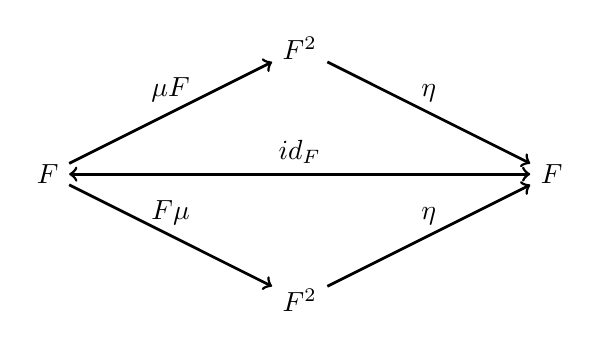
\begin{tikzpicture}[line width=1pt, scale=0.8]
    % Nodes
    \node (A) at (0,0) {$F$};
    \node (B) at (4,2) {$F^2$};
    \node (C) at (4,-2) {$F^2$};
    \node (D) at (8,0) {$F$};
    \draw[->] (A) -- (B) node[midway, above] {$\mu F$};
    \draw[->] (A) -- (C) node[midway, above] {$F \mu$};
    \draw[->] (B) -- (D) node[midway, above] {$\eta$};
    \draw[->] (C) -- (D) node[midway, above] {$\eta$};
    \draw[<->] (A) -- (D) node[midway, above] {$id_F$};
  \end{tikzpicture}

  \item The associativity law:
  For $F\circ F\circ F$ first two $F$ then collapse to $F$
  is the same as collapsing the last two $F$ then collapse to $F$.

  The following diagram commutes:

  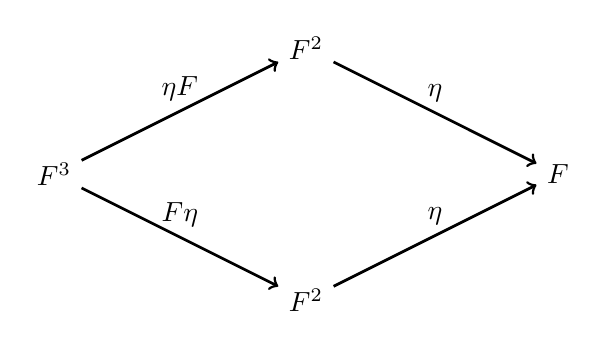
\begin{tikzpicture}[line width=1pt, scale=0.8]
    % Nodes
    \node (A) at (0,0) {$F^3$};
    \node (B) at (4,2) {$F^2$};
    \node (C) at (4,-2) {$F^2$};
    \node (D) at (8,0) {$F$};
    \draw[->] (A) -- (B) node[midway, above] {$\eta F$};
    \draw[->] (A) -- (C) node[midway, above] {$F \eta$};
    \draw[->] (B) -- (D) node[midway, above] {$\eta$};
    \draw[->] (C) -- (D) node[midway, above] {$\eta$};
  \end{tikzpicture}
\end{itemize}

\pagebreak
\section*{Monad in haskell}
Assume we have a category $Hask$ which is the category of haskell types and functions.
We can encode the monad in haskell as follows. But it is hard to implement the monad laws in haskell,
since lack of dependent type.

\begin{minted}{haskell}
data Identity a = Identity a
type NaturalTransformation f g = forall a. f a -> g a
type Compose f g a = f (g a)
class Monad m where
  unit :: NaturalTransformation Identity m
  join :: NaturalTransformation (Compose m m) m
\end{minted}

Some example that violate the monad laws:
Let's define a monad instance for list that violate the monad laws.
([], join, unit)
\begin{minted}{haskell}
join = concat . reverse
unit x = [x]
\end{minted}

  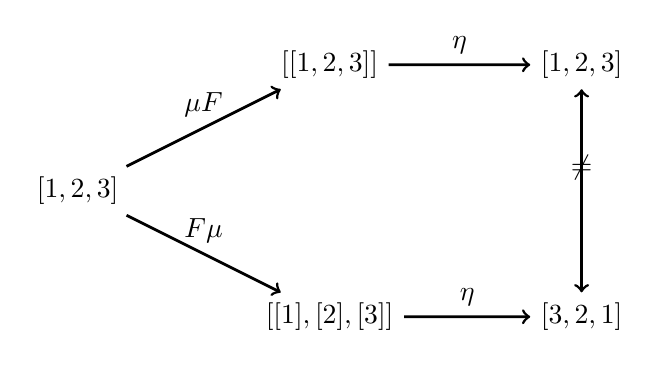
\begin{tikzpicture}[line width=1pt, scale=0.8]
    % Nodes
    \node (A) at (0,0) {$[1,2,3]$};
    \node (B) at (4,2) {$[[1,2,3]]$};
    \node (C) at (4,-2) {$[[1],[2],[3]]$};
    \node (D1) at (8,2) {$[1,2,3]$};
    \node (D2) at (8,-2) {$[3,2,1]$};
    \draw[->] (A) -- (B) node[midway, above] {$\mu F$};
    \draw[->] (A) -- (C) node[midway, above] {$F \mu$};
    \draw[->] (B) -- (D1) node[midway, above] {$\eta$};
    \draw[->] (C) -- (D2) node[midway, above] {$\eta$};
    \draw[<->] (D1) -- (D2) node[midway, above] {$\neq$};
  \end{tikzpicture}


\end{document}